% preamble and style file for M&R lecture slides
\documentclass[11.5pt,sans,english]{beamer}

\usetheme{EastLansing}
\usecolortheme{lily}

\usepackage[most]{tcolorbox}

\usepackage{verbatim}
%\usepackage{ulem}
%\usepackage{fontawesome}
%\usepackage{tikz}
%\usepackage{pifont}
%\usepackage{tabularx}
\usepackage{array,booktabs,xcolor,colortbl,multirow,rotating,amssymb}
%\usepackage{amsmath}
% \usepackage{vwcol}
% \usepackage[T1]{fontenc}

  
\newcommand\vect[1]{\underline{\mathbf{#1}}}
\newcommand\unitvect[1]{\hat{\boldsymbol{#1}}}
%\newcommand\hatdot[1] { \hat{ \dot{ \boldsymbol{#1} } } }

\newtcbox
{\keyc}{on line,arc=2pt, colback=yellow!30!white, colframe=yellow!30!black, before upper={\rule[-3pt]{0pt}{10pt} },boxrule=1pt,boxsep=0pt,left=6pt,right=6pt,top=2pt,bottom=2pt,}

\newtcbox
{\keyb}{on line,arc=1pt, colback=blue!30!white, colframe=blue!30!black, before upper={\rule[-3pt]{0pt}{10pt} },boxrule=1pt,boxsep=0pt,left=6pt,right=6pt,top=2pt,bottom=2pt,}

\newtcbox
{\keyl}{on line,arc=1pt, colback=pink!30!white, colframe=blue!30!black, before upper={\rule[-3pt]{0pt}{10pt} },boxrule=1pt,boxsep=0pt,left=6pt,right=6pt,top=2pt,bottom=2pt,}

\newtcbox
{\keyw}{on line,arc=1pt, colback=red!30!white, colframe=blue!30!black, before upper={\rule[-3pt]{0pt}{10pt} },boxrule=1pt,boxsep=0pt,left=6pt,right=6pt,top=2pt,bottom=2pt,}

\newtcbox
{\keya}{on line,arc=1pt, colback=purple!30!white, colframe=blue!30!black, before upper={\rule[-3pt]{0pt}{10pt} },boxrule=1pt,boxsep=0pt,left=6pt,right=6pt,top=2pt,bottom=2pt,}

\newtcbox[auto counter,number within=section]
{keyf}
{
enhanced,
on line,
  boxsep=0pt,
  left=6pt,right=6pt,top=2pt,bottom=2pt,
  arc=5pt,
  boxrule=1pt,
  rightrule=38pt,
colback=green!10!white, 
colframe=green!50!black, 
title=\thetcbcounter,
detach title,
overlay unbroken and first ={
    \node[%rotate=90,
          %minimum width=1cm,
          anchor=south,
          font=\sffamily\bfseries\tiny,
          %yshift=-10pt,
          yshift=-5pt,
          xshift=-20pt,
          white]
    at (frame.east) {\thetcbcounter};
  }
}


\usepackage{xcolor}

%\usepackage{hyperref}
%\hypersetup{
%  pdfauthor={Lily Asquith},
%  urlcolor=blue,
%  colorlinks=true,
%  linkcolor=blue,
%  bookmarks=true
%}

%---------------------------------------------%
%              LILY'S COLOURS           %
%---------------------------------------------%
\definecolor{Wash}{RGB}{204,204,204}
%\definecolor{Pinky}{RGB}{254,200,254}%violet
\definecolor{Pinky}{RGB}{219,	240,	253}%violet
\definecolor{Bluey}{RGB}{0,190,255}%deep sky blue
\definecolor{DarkGrey}{RGB}{28,66,137}%dar grey
\definecolor{SussexWhite}{RGB}{253,255,254}%dar grey
\definecolor{LightGray}{RGB}{184,184,255}
\definecolor{YesGreen}{RGB}{0,128,0}
\definecolor{NoRed}{RGB}{250,0,0}



\definecolor{myred}{RGB}{255,153,153}
\definecolor{myorange}{RGB}{255,204,153}
\definecolor{myyellow}{RGB}{255,255,153}
\definecolor{mygreen}{RGB}{153,255,153}
\definecolor{mycyan}{RGB}{153,255,255}
\definecolor{myblue}{RGB}{153,204,255}
\definecolor{myviolet}{RGB}{153,153,255}
\definecolor{mypurple}{RGB}{204,153,255}
\definecolor{mypink}{RGB}{255,204,255}
\definecolor{mycoral}{RGB}{255,153,204}

%-----------------------------------------------------%
%              LILY'S COLUMN TYPES          %
%-----------------------------------------------------%
\newcolumntype{a}{>{\raggedright\arraybackslash}l}	
\newcolumntype{q}{>{\raggedright\arraybackslash}m{8cm}} 

%--------------------------------------------%
%              LILY'S SYMBOLS          %
%--------------------------------------------%
\newcommand{\dfinger}{\large{\textcolor{black}{\ding{43}}}\scriptsize}
\newcommand{\dstar}{\large{\textcolor{black}{\ding{76}}}\scriptsize}
\newcommand{\dwrite}{\large{\textcolor{black}{\ding{45}}}\scriptsize}
\newcommand{\ddiamond}{\small{\textcolor{DarkGrey}{\ding{117}}}\scriptsize}
\newcommand{\ddiamondwhite}{\small{\textcolor{SussexWhite}{\ding{117}}}\scriptsize}
\newcommand{\experiment}{\small{\textcolor{magenta}{\faCogs }}\scriptsize}
\newcommand{\watchit}{\textcolor{blue}{ \faYoutube}}


\makeatletter
\newcommand\notsotiny{\@setfontsize\notsotiny{6.5}{7.5}}
\makeatother


% 
\title[ Intro to Quantum Physics]{Intro to Quantum Physics F3241}
%\subtitle{\textbf{Part 4: The Photoelectric Effect}}
\author[Dr Lily Asquith (Lily)]{ Dr Lily Asquith (Lily)}
\date[Week 5]{ Week 5}
\logo{

\includegraphics[width=1.5cm]{../../utils/uslogo.jpg}
}


\begin{document}


\begin{frame}
\titlepage
\end{frame} 


\section{I2Q Part 5: Compton Scattering}

 
 \begin{frame}{Warm up!}
\small

$E= hf= \frac{hc }{\lambda }$\\[2ex]

$E^2 = m^2 c^{4} +p^2c^2 $\\[2ex]

$\frac{ h c}{ \lambda} = pc$\\[2ex]

Momentum $p = \frac{ h}{ \lambda } $ \\[2ex]
%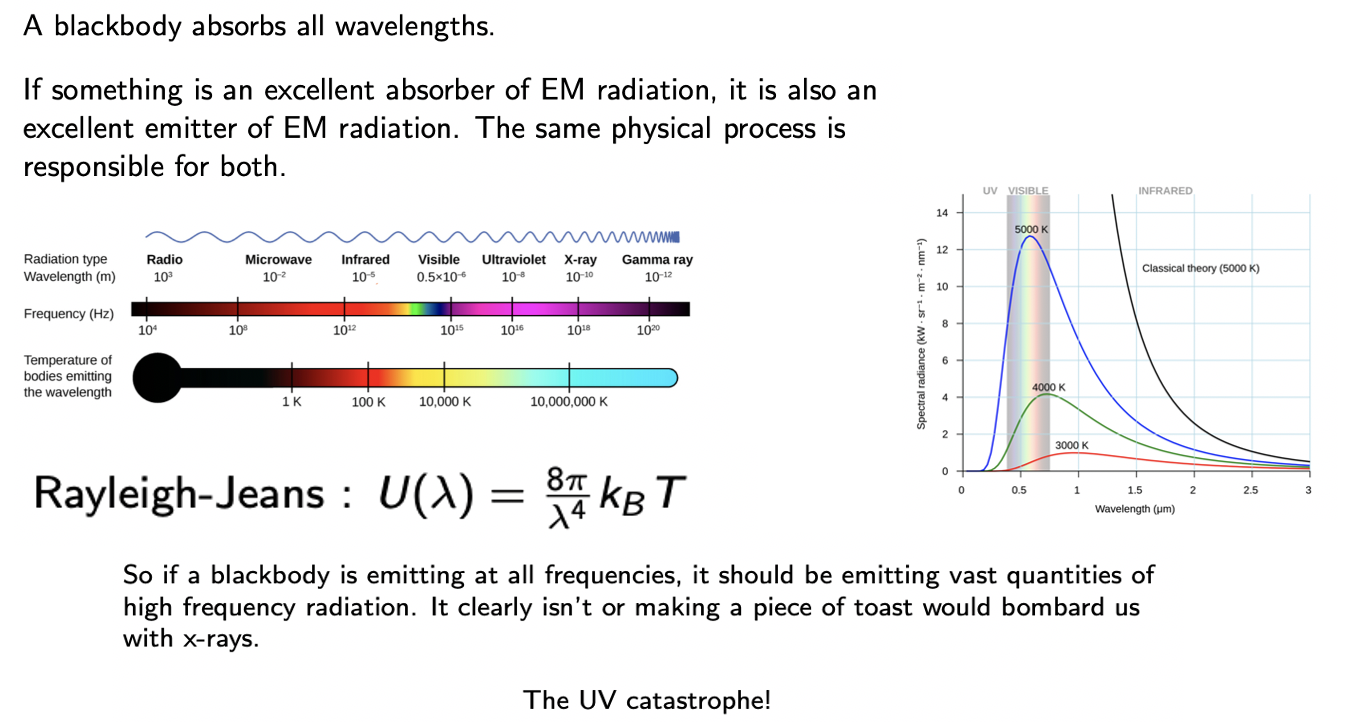
\includegraphics[scale=0.45]{uvcatas-recap}

What about electrons?\\
\end{frame}


 %-----------------------------------------------------------%
 % LECTURE 1
 %---------------------------------------------------------

\subsection{Diffraction \& x-rays}


%\begin{frame}{Diffraction \& x-rays}
%\small
%Shining light on a screen with a hole in it is really strong evidence that light is an EM wave.\\[1ex]
%
%Remember Hertz showed this for radio waves, and then also sparked the photoelectric experiment, which makes radiation look like it is made of particles rather than waves...\\
%
%You will do wave mechanics next term with David Seery, but let's get a little taster now, just enough that we can  for a sensible thought process about what is happening.\\
%
%All waves interfere. If you go to a gig, try slowly moving horizontally between the stage and the sound rig. You will notice a change in both the quality and volume depending on where you are positioned. (Sound waves are not the same as EM waves: they are pressure waves).\\
%
%For EM waves (aka radiation) they leave a source in every direction, spherically.\\
%
%If we mess with that by placing a straight line in its path, we will cause the radiation to interfere with itself\\
%
%At a screen place some distance away, what is happening?\\
%
%When light shines on a surface, we can see it. It reflects off the surface and back to our eyes. What does that mean? Is it the same light?\\
%
%Why does this jumper look blue?\\
%
%Different things can happen when light is incident on a material. \\
%
%The light is scattered from the material\\
%- if it doesn't have enough energy to free an electron this will always happen. It will collide with an electron and conservation of energy means it must be scattered back in some direction.
%- if it does have enough energy to free an electron this can also happen. It will pay the tax, free the electron, and then take the remaining energy off with it.\\
%
%The light is absorbed by the material, having its entire energy redistributed as a tax to free the bound electron, and the freed electron energy.\\
%
%The light is absorbed by the material, but instead of freeing a loosely bound electron, it makes a tightly bound one less loosely bound (excited). This guy will immediately drop back down into its unexcited ground state, and that energy will be released as light of a characteristic frequency.
%
%The light passes through the material, as if it were not there. Or some of it does...
%
%
%
%%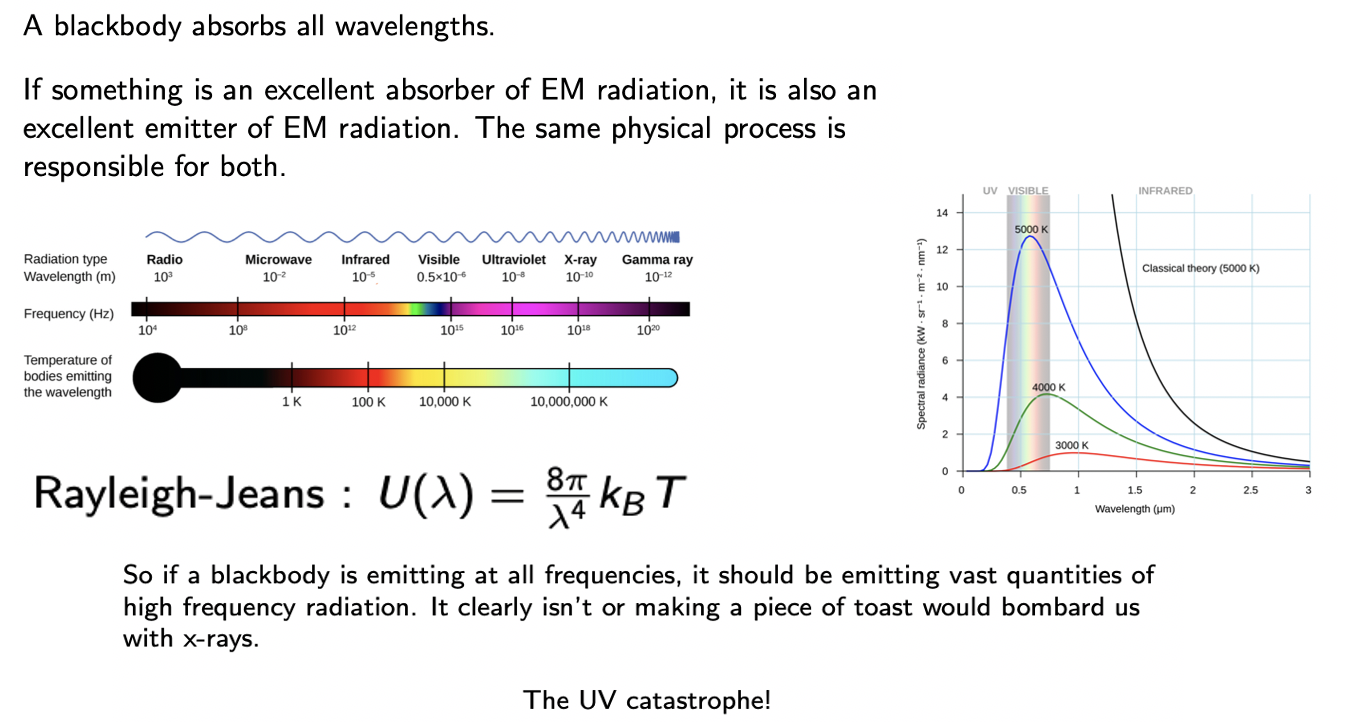
\includegraphics[scale=0.45]{uvcatas-recap}
%\end{frame}

\begin{frame}{Diffraction}{Diffraction}
\small
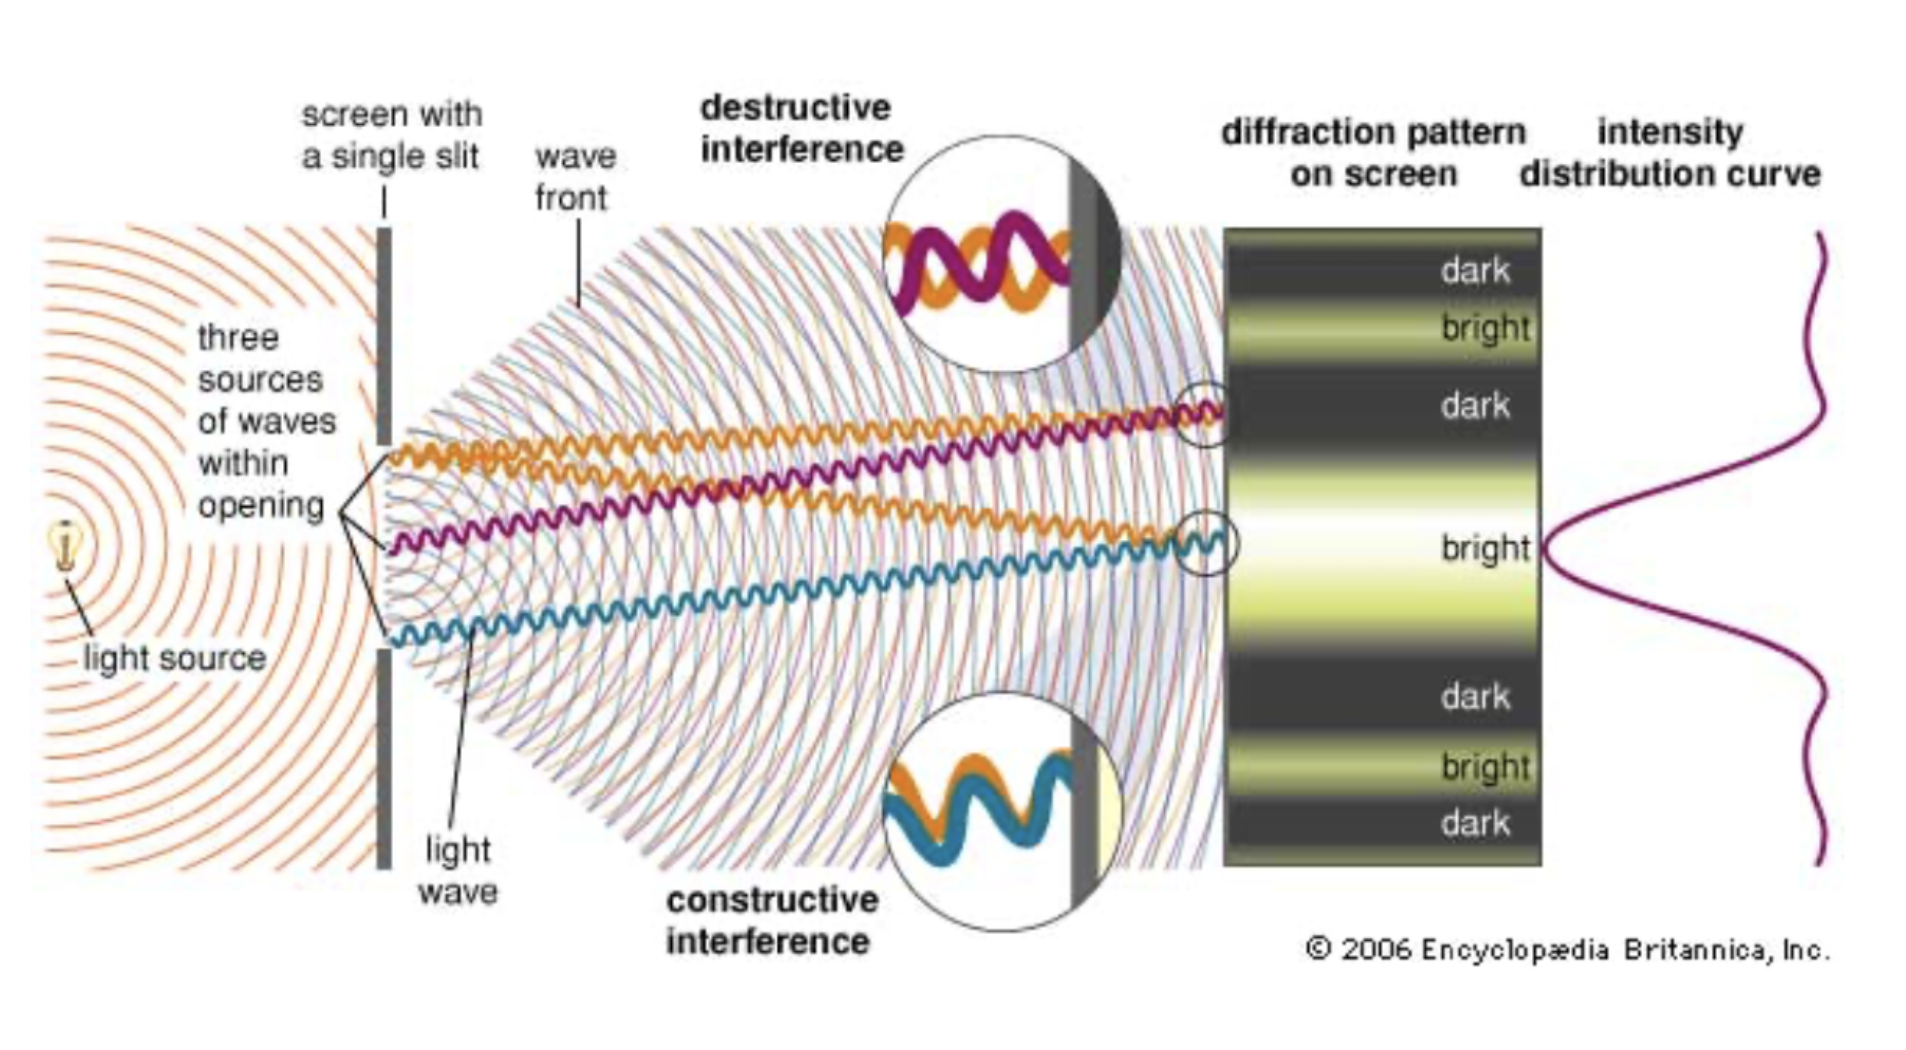
\includegraphics[scale=0.3]{diff1}


\end{frame}


\begin{frame}{Bragg's Formula for Constructive Interference}
\small
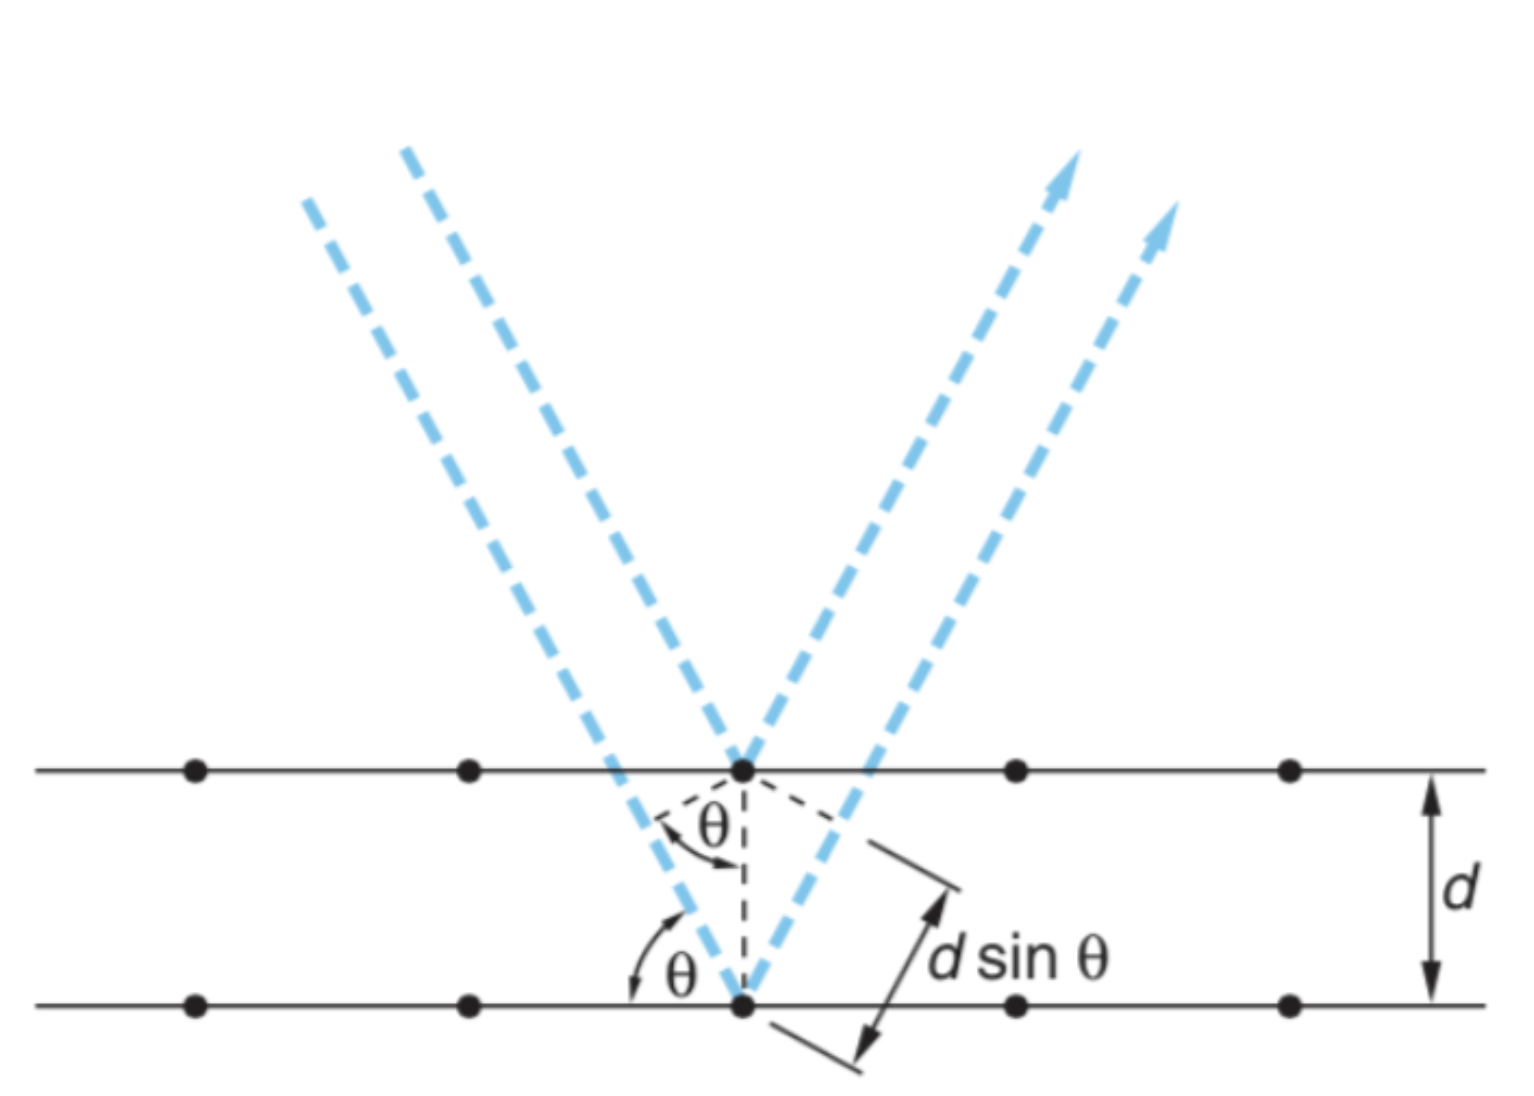
\includegraphics[scale=0.3]{2dsintheta}


\end{frame}


\begin{frame}{The Discovery of X-rays}
\small
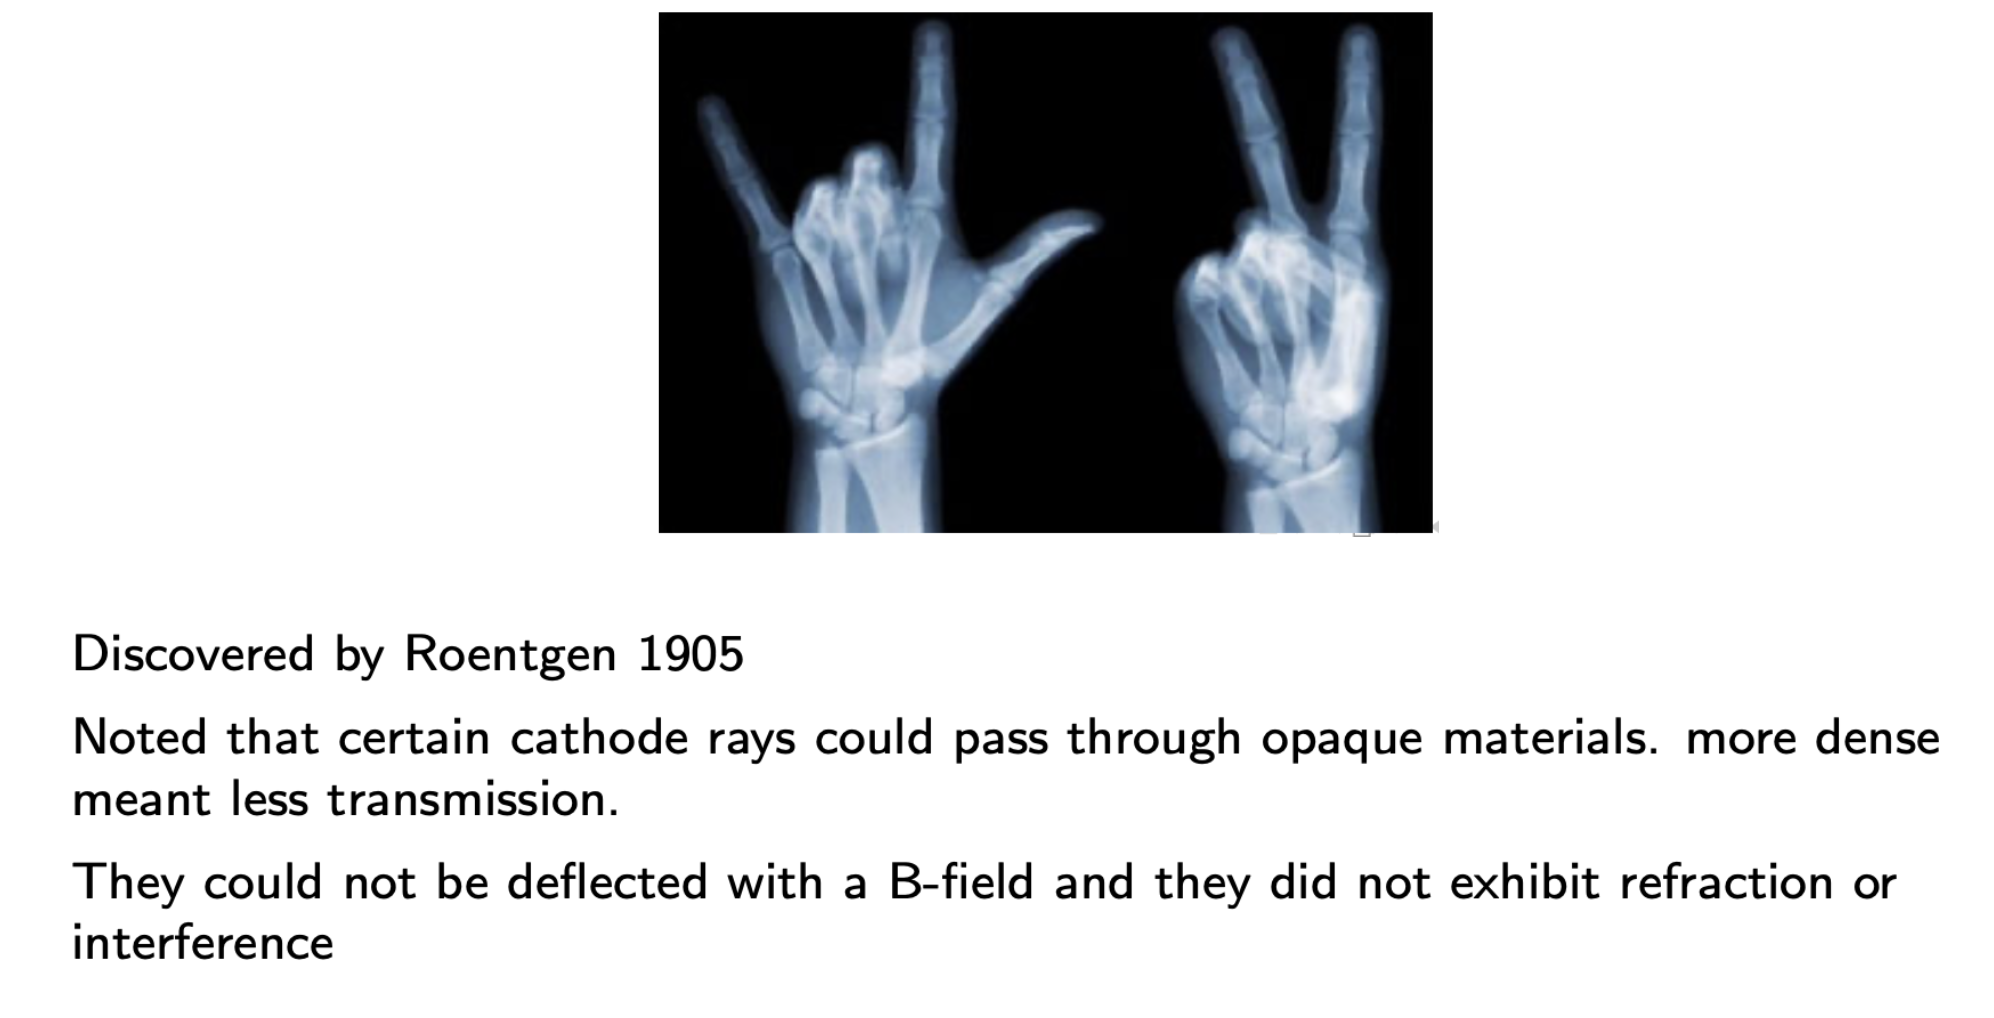
\includegraphics[scale=0.3]{xrays1}

\end{frame}


\begin{frame}{How are x-rays produced?}
\small
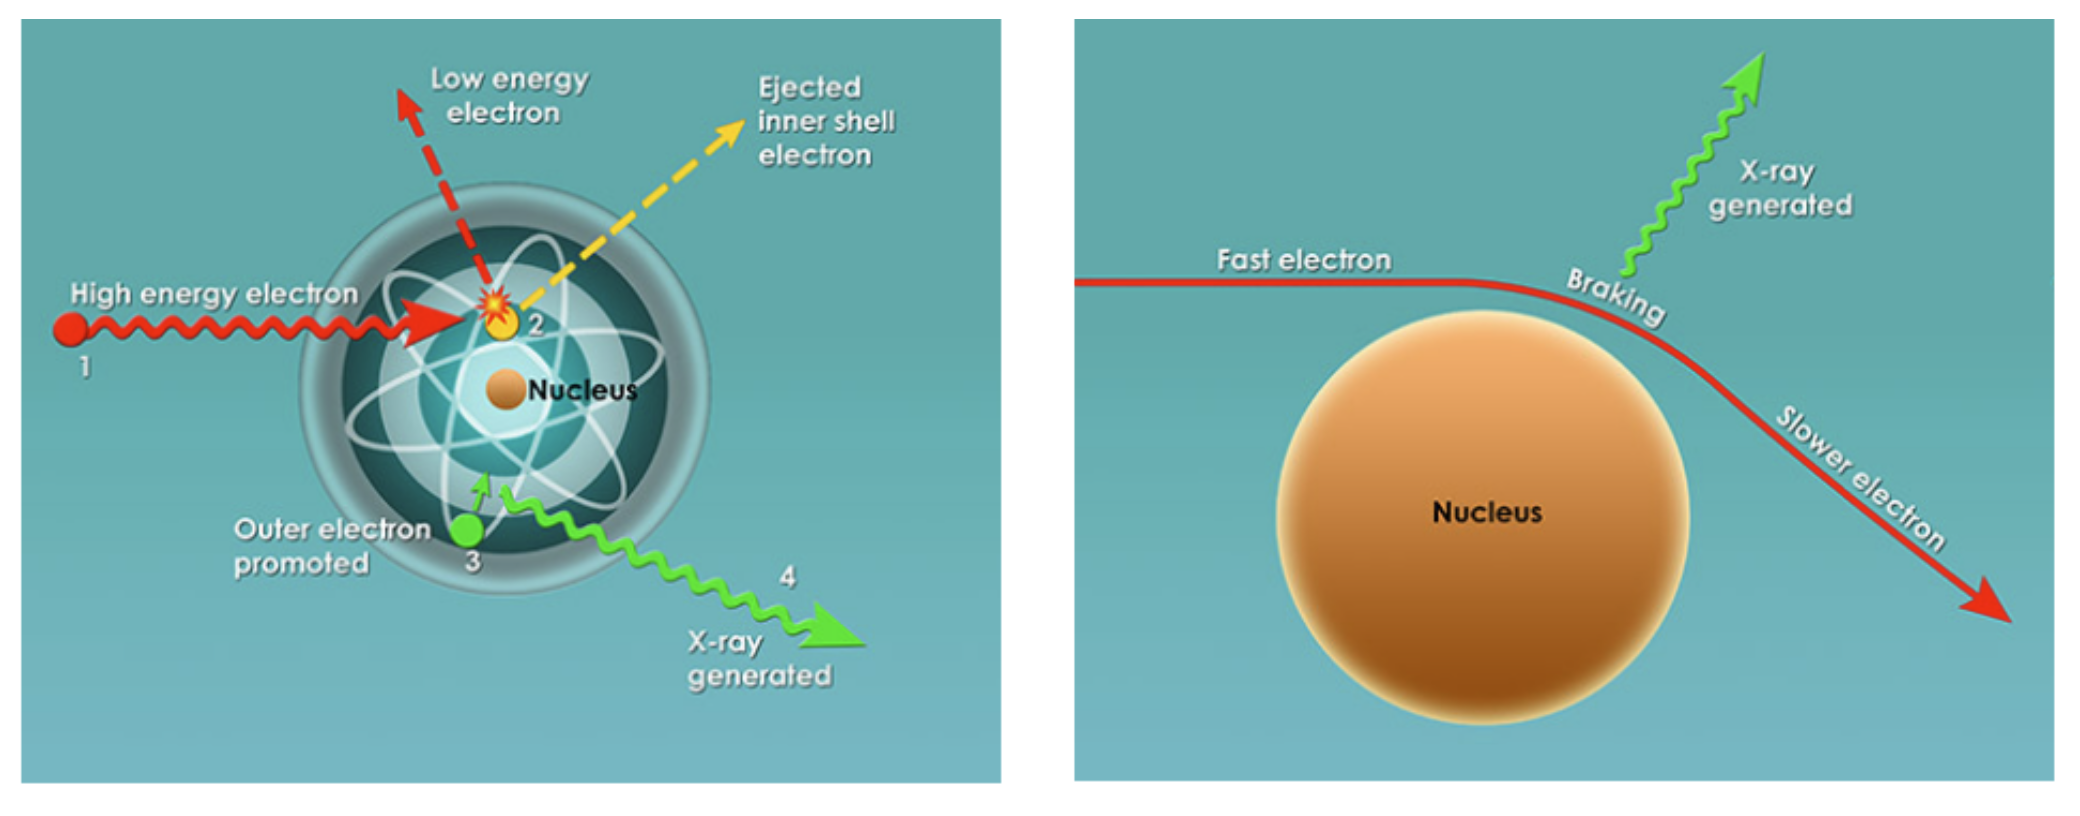
\includegraphics[scale=0.3]{xrayprod}

\end{frame}


\begin{frame}{Diffraction Gratings}
\small
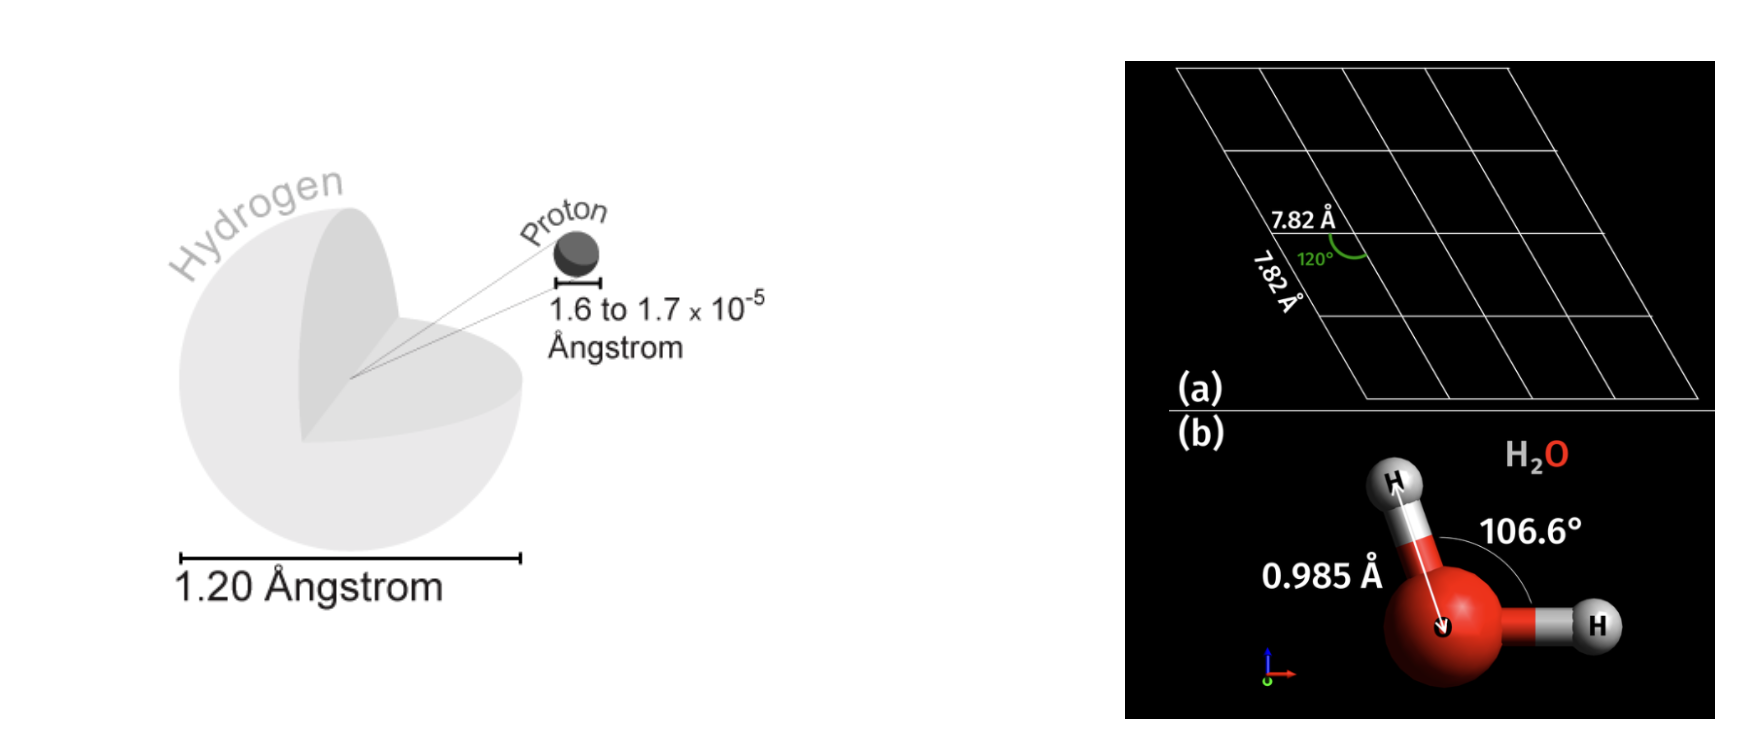
\includegraphics[scale=0.3]{grating}


\end{frame}




\begin{frame}{The Compton Experiment}
\small
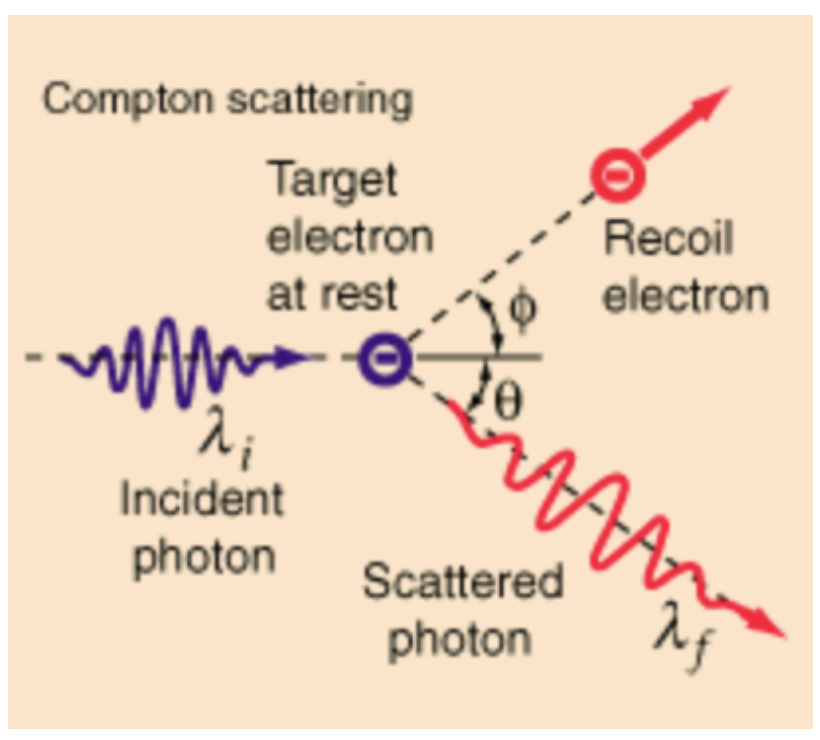
\includegraphics[scale=0.3]{compton1}


\end{frame}

\begin{frame}{Compton's Measurements}
\small
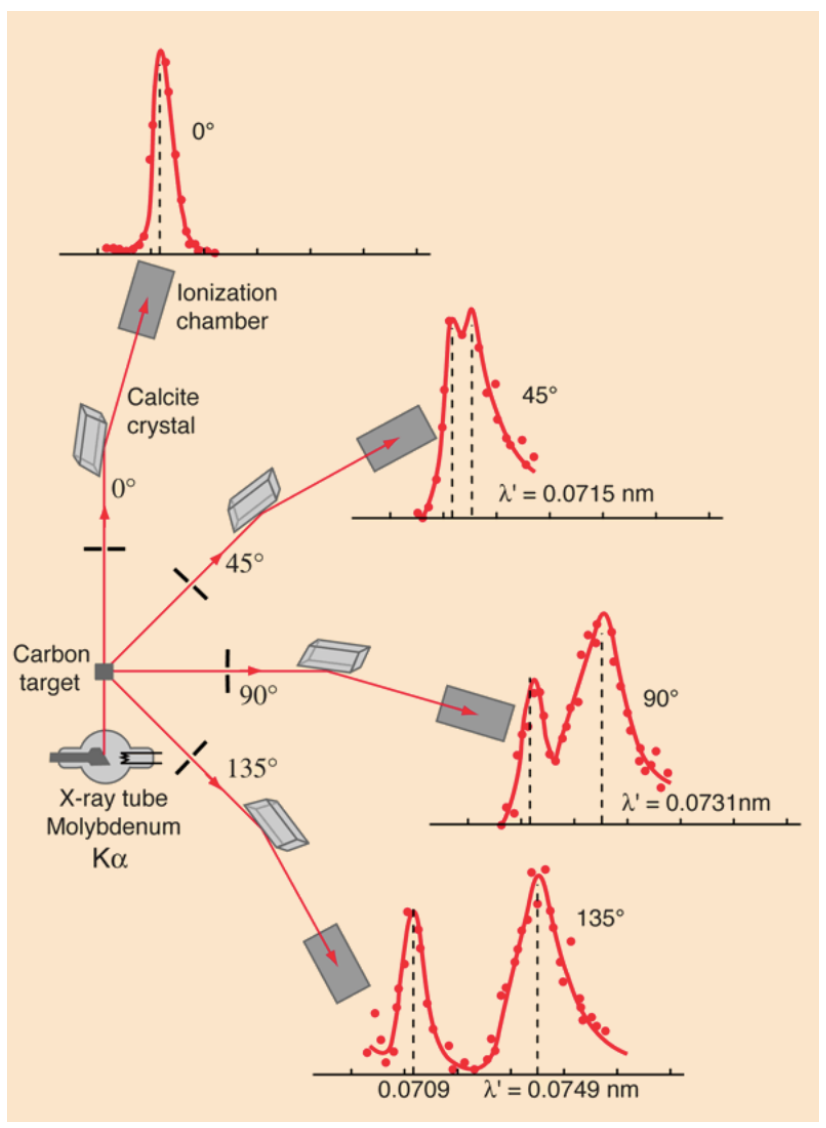
\includegraphics[scale=0.3]{compton2}


\end{frame}


\begin{frame}{Modern Picture}
\small
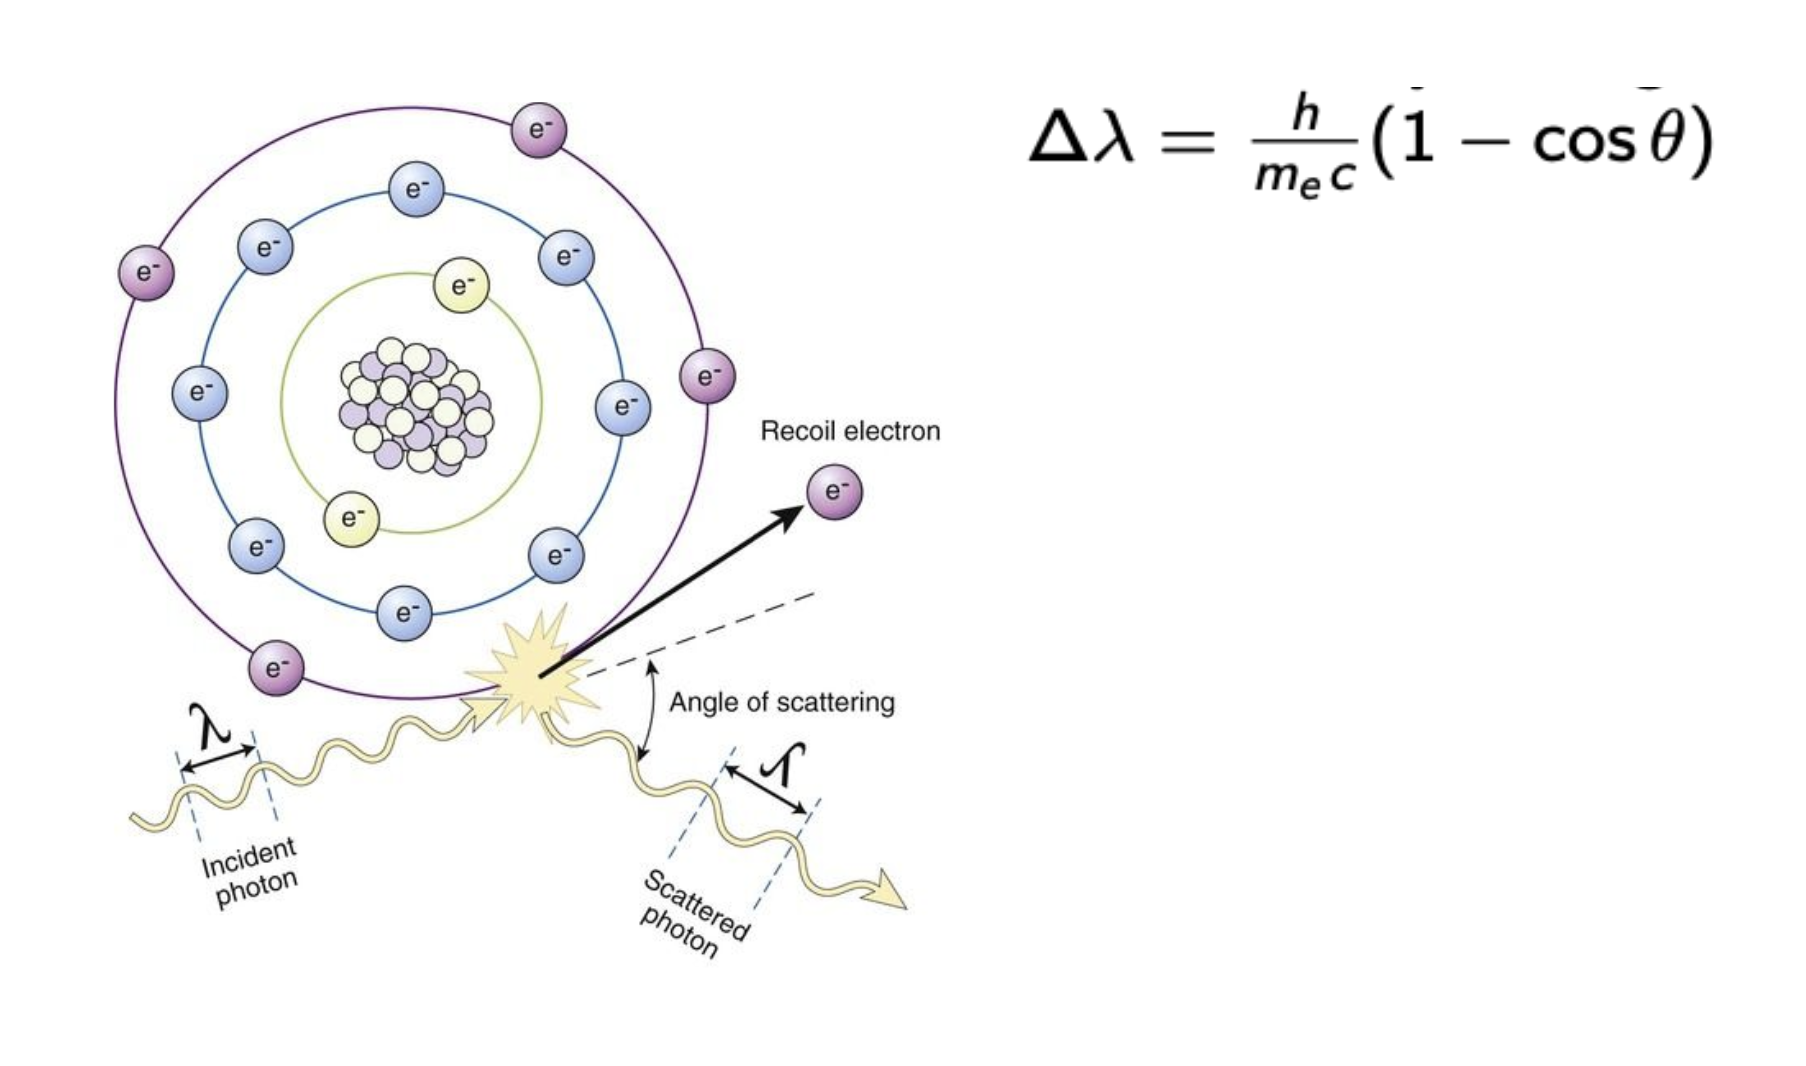
\includegraphics[scale=0.3]{cartoon}


\end{frame}



\begin{frame}{Key formulae}
\small
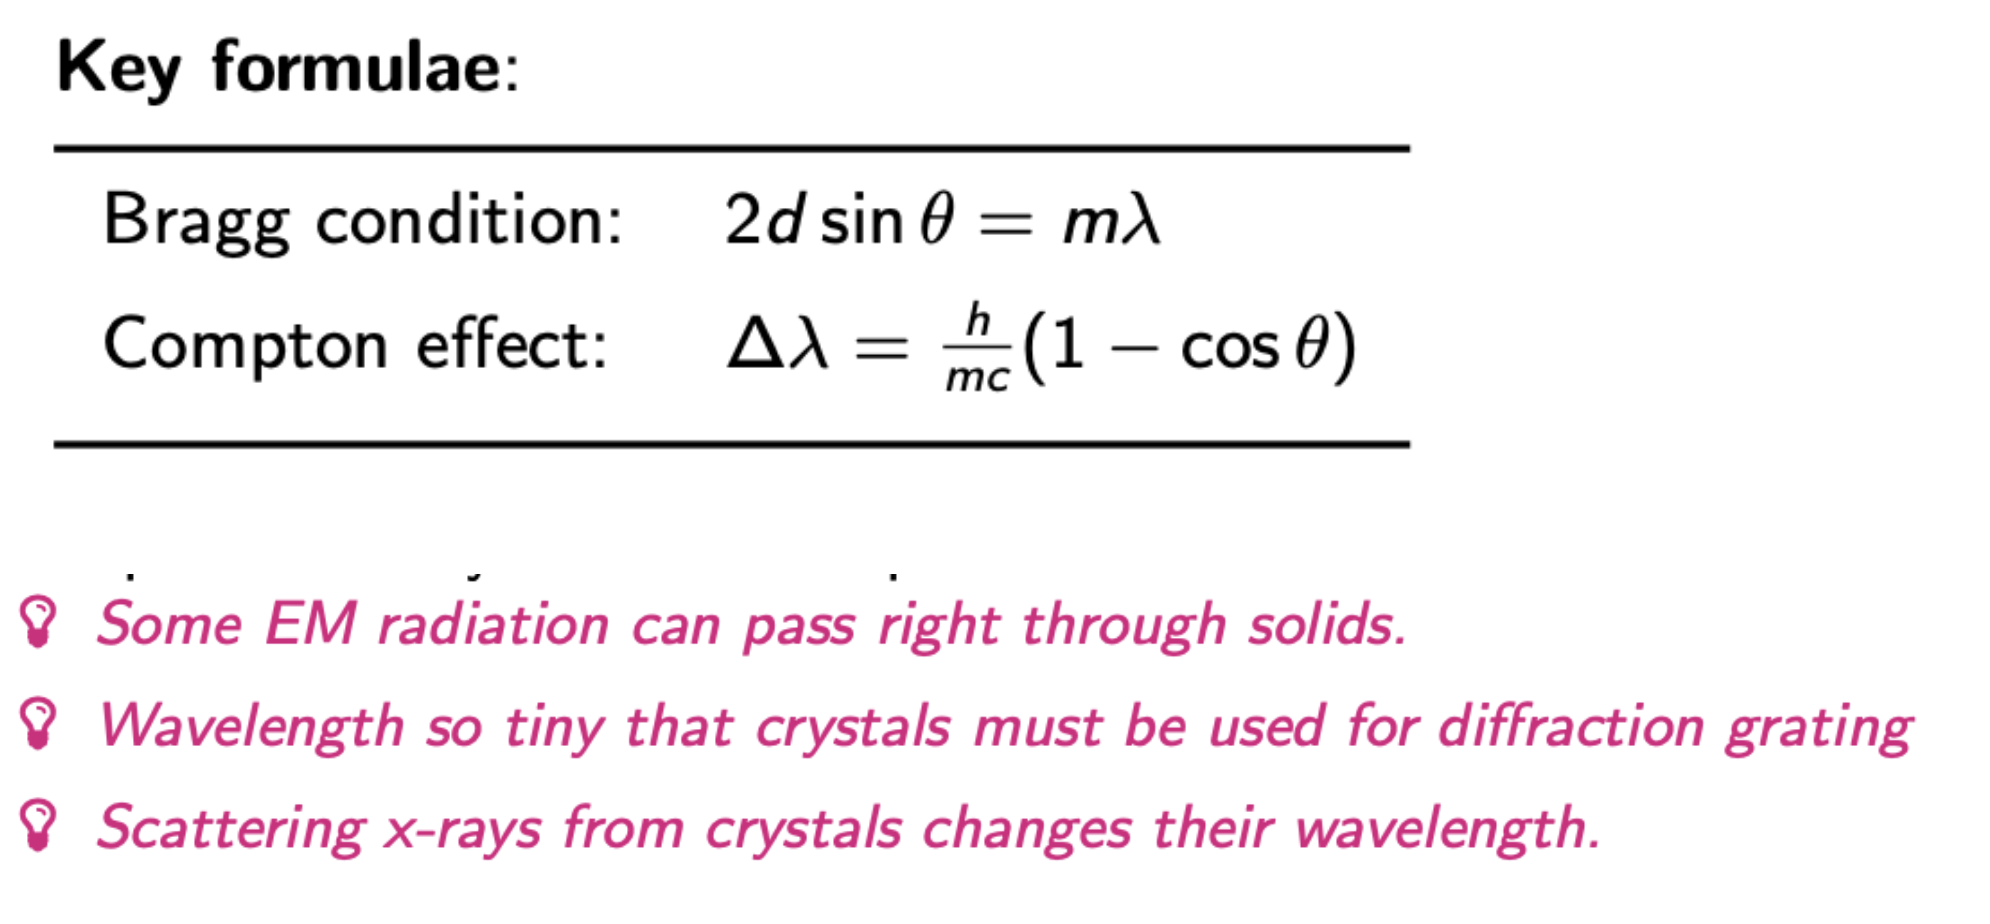
\includegraphics[scale=0.3]{keyform}


\end{frame}


\begin{frame}{How radiation interacts with matter}
\small
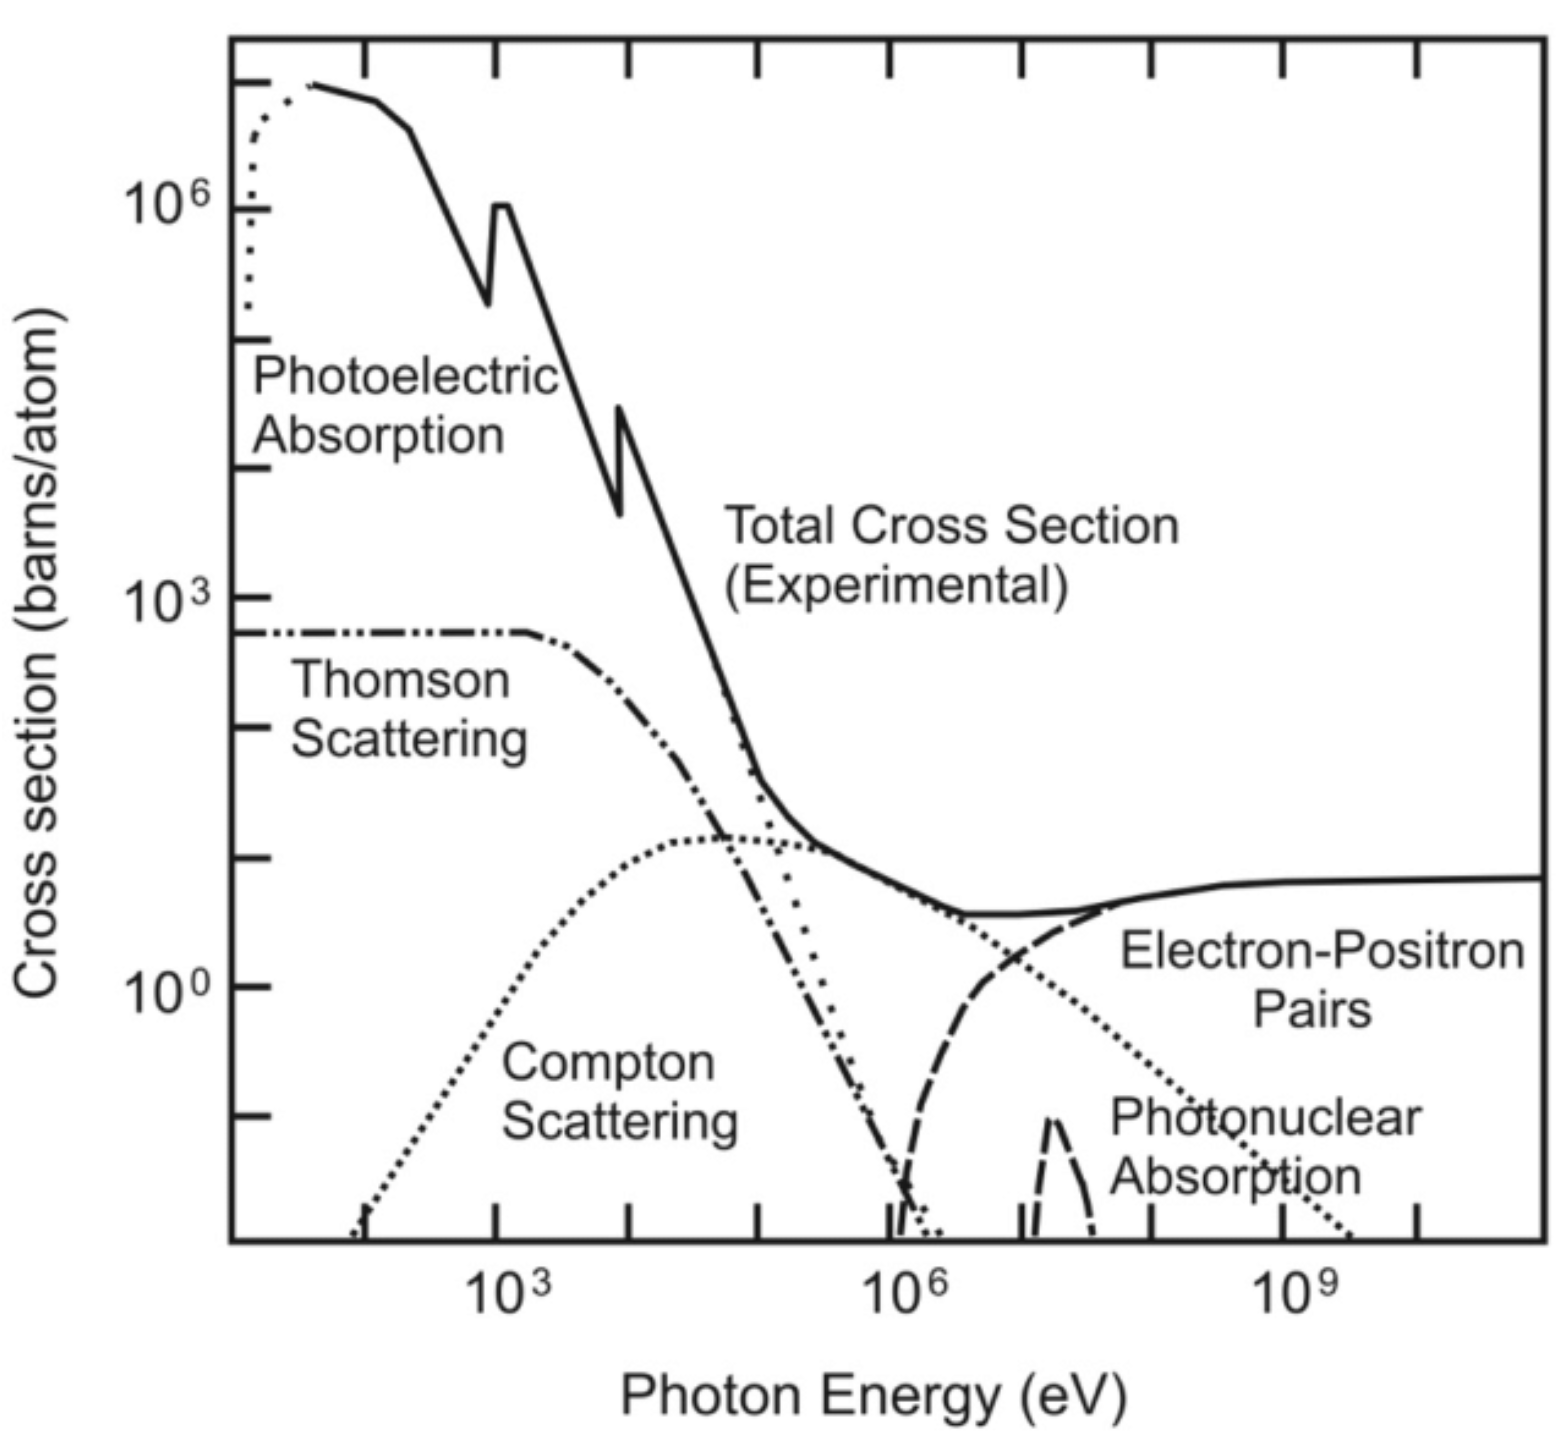
\includegraphics[scale=0.3]{cross-secs}


\end{frame}



\begin{frame}{Barns}
\small
The diameter of a Uranium atom is 138.5 pm. What is its cross-sectional area, in barns?\\[1ex]
\vspace{10cm}

\end{frame}



\begin{frame}{Exercise}
\small
An x-ray with energy 124 keV is incident on a an Al target with loosely bound electrons. \\[4ex]

What is the wavelength of the x-ray photons, $\lambda_i$?\\[4ex]

What is the wavelength of the scattered photons, $\lambda_f$, measured at $\theta = 90^{\circ}$ from the incoming direction?\\[4ex]


What is the energy $E_{f}$ of the scattered photons?\\[4ex]

\end{frame}

\begin{frame}{Exercise for homework}
\small
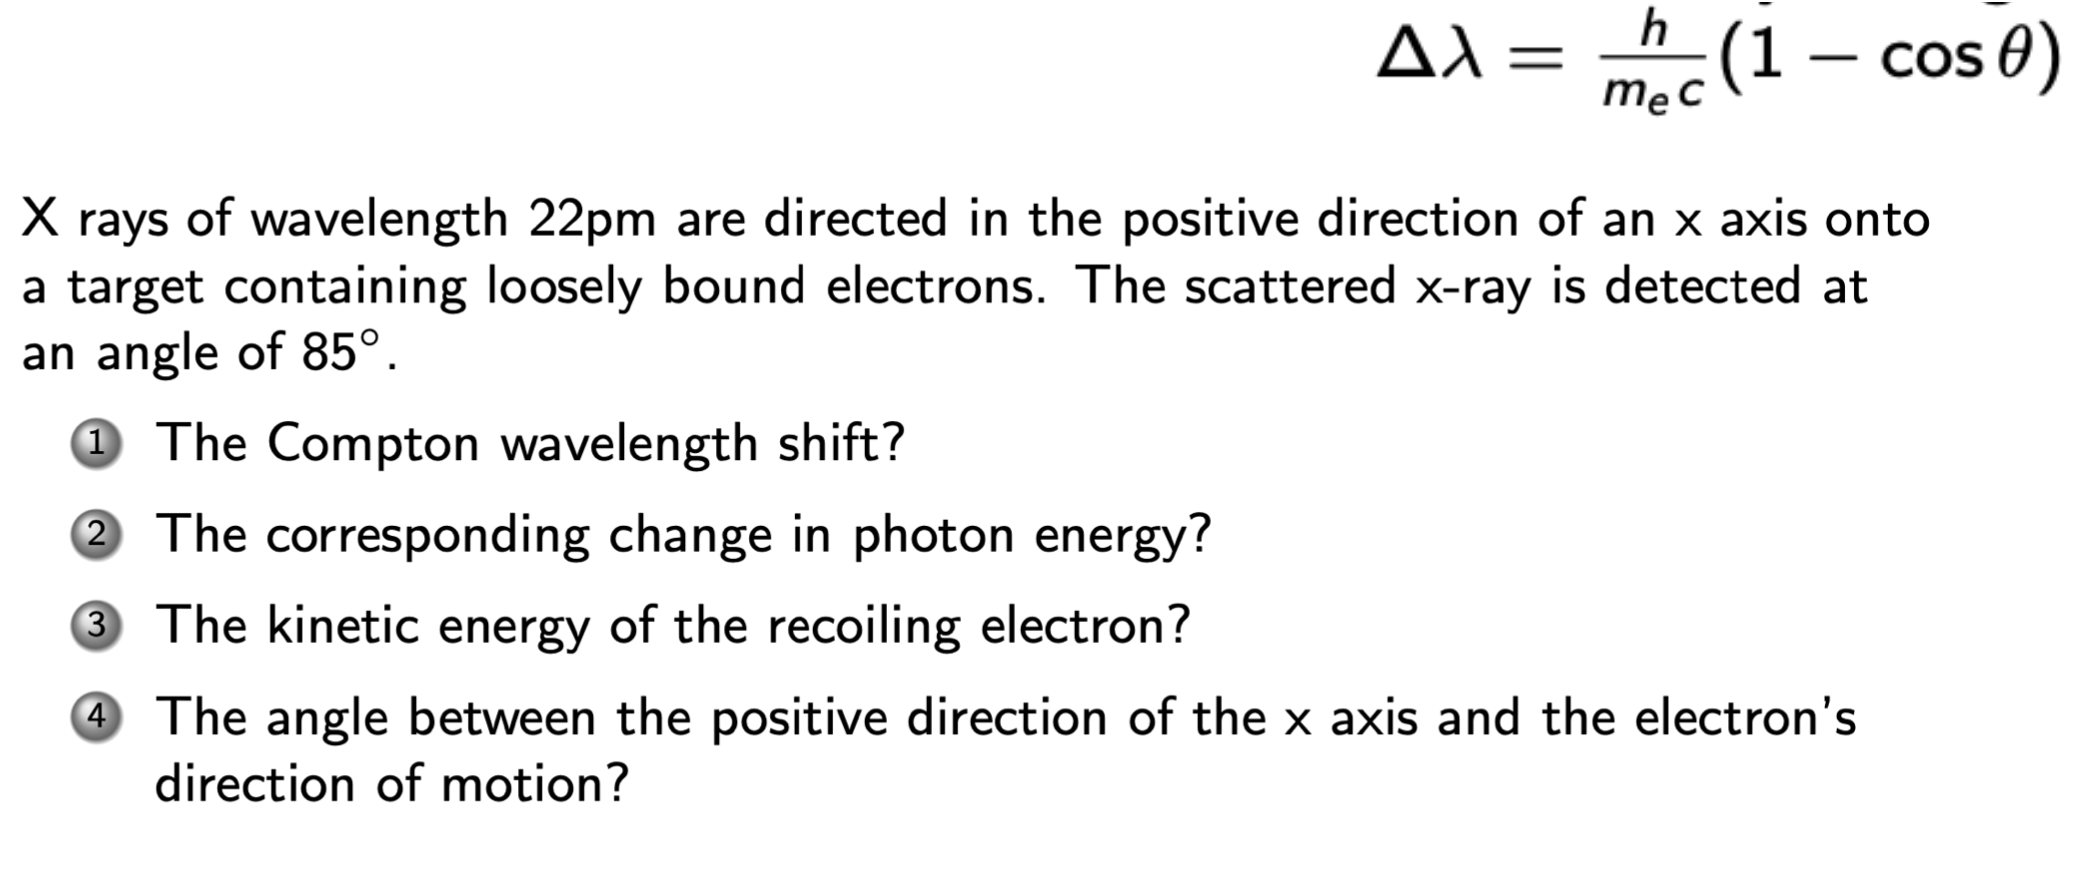
\includegraphics[scale=0.3]{shift}


\end{frame}


\end{document}